\documentclass[a4paper, 11pt]{article}

% \usepackage[''paramètre'']{inputenc}
\usepackage{graphicx}
\usepackage[french]{babel}
\usepackage[T1]{fontenc} 
\usepackage[a4paper, margin=2.5cm]{geometry}
\usepackage{amsmath}
\usepackage{float}
\usepackage{caption}

\frenchsetup{StandardItemLabels=true}

\title{Projet MNI : \\ Modèle de Kuramoto \& Modèle FPUT}
\author{A. Cremel-Schlemer (3800159) \\ L. Jonkisz (28708367) \\ M. Panet (28705836)}
\date{30 Novembre 2023}

\begin{document}

\maketitle
\section{Le modèle de Kuramoto}
\subsection*{Question Préambule}
\begin{align*}
    \theta_{i} &=\omega_{i} + \displaystyle \sum_{j=1}^{N} \frac{K}{N} \sin(\theta_{j} - \theta_{i}) \\
    &=\omega_{i} +  \frac{K}{N} \displaystyle \sum_{j=1}^{N} \bigg[ sin(\theta_{j})\cos(\theta_{i}) - \cos(\theta_{j})\sin(\theta_{i}) \bigg] \\
   &=\boxed{\omega_{i} +  \frac{K}{N} \bigg[ \cos(\theta_{i}) \displaystyle \sum_{j=1}^{N} \sin(\theta_{j}) -\sin(\theta_{i}) \displaystyle \sum_{j=1}^{N}\cos(\theta_{j})\bigg] } \refstepcounter{equation}\tag{\theequation}
\end{align*}

or on a d'autre part : 
\begin{equation*}
    R e^{i\Psi} = \frac{1}{N} \displaystyle \sum_{i=1}^{N} e^{i\theta_{i}}
\end{equation*}

\begin{equation*}
    NR \cos (\Psi) + i NR \sin (\Psi)  = \displaystyle \sum_{i=1}^{N} \cos(\theta_{i}) + i \sin(\theta_{i}) 
\end{equation*}

par identification : 

\begin{align}
 \boxed{ NR \cos (\Psi) =  \displaystyle \sum_{i=1}^{N} \cos(\theta_{i}) } \\
 \boxed{ NR \sin (\Psi) =  \displaystyle \sum_{i=1}^{N} \sin(\theta_{i}) }
\end{align}


alors on remplace dans (2) et (3) dans (1) : 

\begin{align*}
    \theta_{i} =\omega_{i} +  KR \bigg[\sin(\Psi)\cos(\theta_{i}) -\cos(\Psi)\sin(\theta_{i})\bigg]
\end{align*}
enfin
\begin{align*}
    \boxed{\theta_{i} =\omega_{i} +  KR\sin(\Psi - \theta_{i})}
\end{align*}

\subsection*{Question 1}
\begin{figure}[H]
    \begin{minipage}[c]{0.49\linewidth}
        \centering
        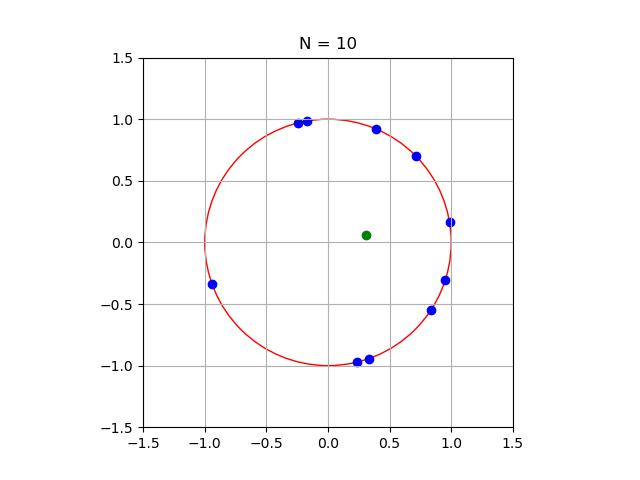
\includegraphics[width=\textwidth]{pics/kura1_10.jpg}
    \end{minipage}\hfill
    \begin{minipage}[c]{0.49\linewidth}
        \centering
        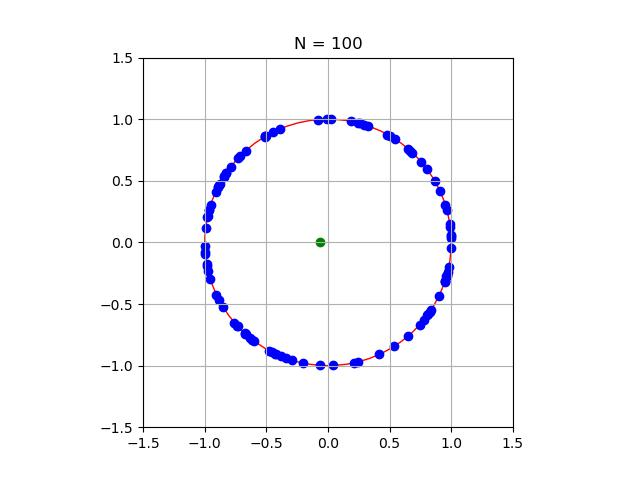
\includegraphics[width=\textwidth]{pics/kura1_100.jpg}
    \end{minipage}
    \caption{Représentation des Oscillateurs pour deux $N$ différents}
\end{figure}

\subsection*{Question 2}
\begin{figure}[H]
    \centering
    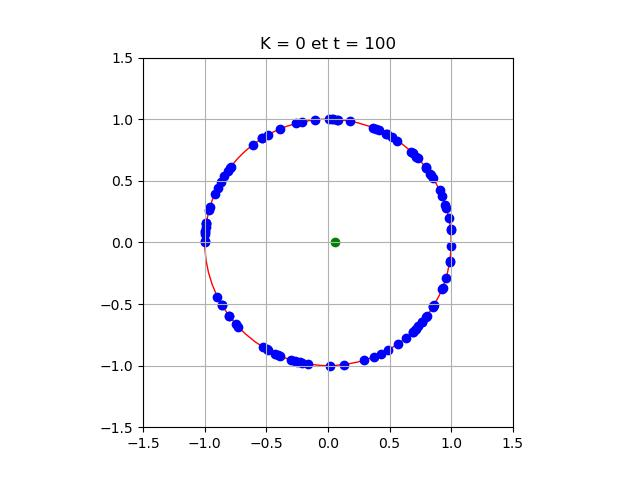
\includegraphics[width=0.49\linewidth]{pics/kura2_100.jpg}
    \caption{Représentation des Oscillateurs à $t=100$}
\end{figure}

\subsection*{Question 3}
Pour $K=0$, on remarque que les phases des l'oscillateurs sont réparties aleatoirement sur l'ensemble $[-\pi, \pi]$. Il n'y a donc aucune synchronisation entre ces oscillateurs. Au contraire, à $K=2$, les phases se regroupent et converge vers une même valeur. Ce phénomène traduit une synchronisation des oscillations.
\begin{figure}[H]
    \centering
    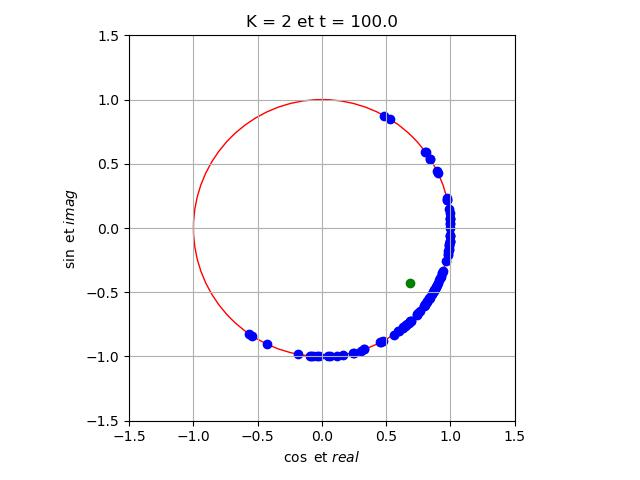
\includegraphics[width=0.49\linewidth]{pics/kura3_100.jpg}
    \caption{Représentation des Oscillateurs à $t=100$ pour $K=2$}
\end{figure}


\subsection*{Question 4}
Nos résultats restent très bruités et nécessited'être répétés afin de réduire l'impact de l'aléatoire.
Cependant, on remarque deux modes de fonctionnement distincts :
\begin{itemize}
    \item Pour $K \leq 1.6$, les modes sont non synchronisés avec $r$ qui reste inférieur à $0.5$.
    \item Pour $K > 1.6$, les modes sont ici synchronisées et les valeurs de $r$ sont bien plus élevées et tendent vers $1$.
\end{itemize}
\begin{figure}[H]
    \centering
    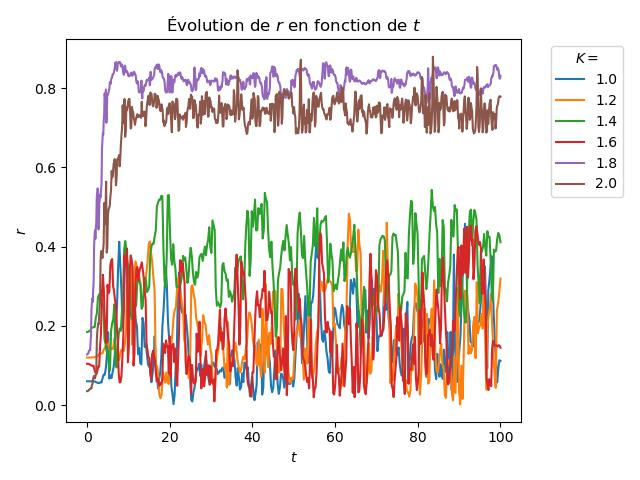
\includegraphics[width=0.6\linewidth]{pics/kura4.jpg}
    \caption{Evolution temporelle de la valeur absolue du terme d'ordre complexe.}
\end{figure}

\subsection*{Question 5}
On remarque que la tendance de $r(K)$ est difficile à interpreter à cause du bruit lié aux fluctuations aléatoires. On voit, néanmoins, qu'elle croit globalement.
\begin{figure}[H]
    \centering
    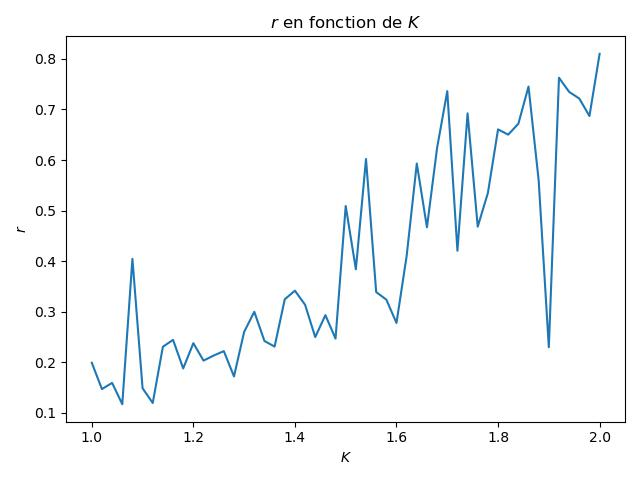
\includegraphics[width=0.5\linewidth]{pics/kura5.jpg}
    \caption{Evolution de $r$ en fonction de $K$ sans répétition.}
\end{figure}

\subsection*{Question 6}
\begin{figure}[H]
    \centering
    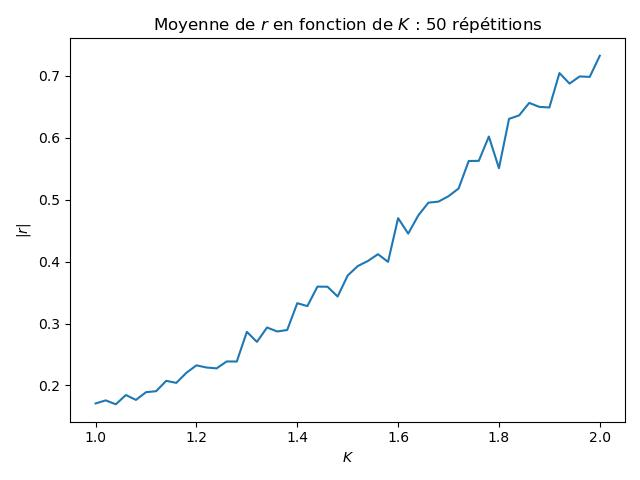
\includegraphics[width=0.5\linewidth]{pics/kura6_50.jpg}
    \caption{Evolution de $r$ en fonction de $K$ avec répétition.}
\end{figure}

\subsection*{Question 7}
\begin{figure}[H]
    \centering
    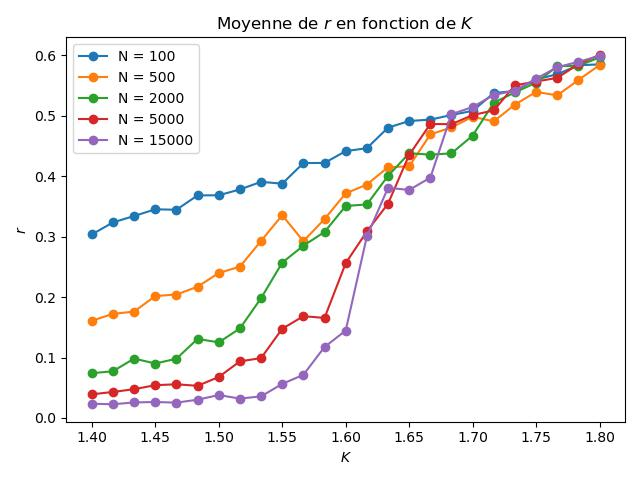
\includegraphics[width=0.5\linewidth]{pics/kura7.jpg}
    \caption{Evolution de $r$ en fonction de $K$ avec répétition et avec différentes tailles de systèmes.}
\end{figure}

\subsection*{Question 8}
\begin{figure}[H]
    \centering
    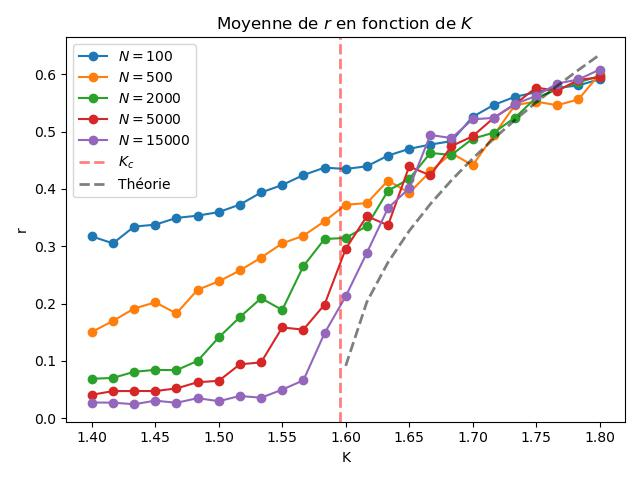
\includegraphics[width=0.5\linewidth]{pics/kura8.jpg}
    \caption{Evolution de $r$ en fonction de $K$}
\end{figure}

\subsection*{Question 9}
\begin{equation*}
    r = \sqrt{\frac{-16 (K-K_{c})}{\pi K_{c}^{4} g"(0)}}
\end{equation*}
avec : 
\begin{equation*}
    K_{c} = \frac{2}{\pi} \sqrt{2\pi} = \frac{4}{\sqrt{2\pi}}
\end{equation*}
 et 
 \begin{equation*}
    g"(0) = -\frac{1}{\sqrt{2\pi}}
\end{equation*}
on a : 
\begin{equation*}
    \boxed{r = \sqrt{ \frac{8 (K-K_{c})}{ K_{c}^{3}}}}
\end{equation*}
Fonction de Bessel : 
\begin{equation*}
    I(n,x) = \displaystyle \sum_{p=0}^{\infty} \frac{{(-1)}^{p}}{p!(p+n)!} {\Bigl( \frac{x}{2}\Bigl)}^{2p+n}
\end{equation*}
On fait le DL en $y$ de : 
\begin{align*} \label{eq:DL}
r &= \frac{y\sqrt{2\pi}}{4} e^{-\frac{y^{2}}{4}} \bigg[ I(0,\frac{y^{2}}{4})+I(1,\frac{y^{2}}{4}) \bigg] \refstepcounter{equation}\tag{\theequation} \\
&= \frac{y\sqrt{2\pi}}{4} \bigg[ 1 - \frac{{y}^{2}}{4} + o({{y}^{3}}) \bigg] \bigg[ \bigl( 1 + o({{y}^{3}}) \bigl) + \bigl( \frac{{y}^{2}}{8} + o({{y}^{3}}) \bigl) \bigg] \\
&= \frac{y\sqrt{2\pi}}{4} \bigg[ 1 - \frac{{y}^{2}}{8} + o({{y}^{3}}) \bigg] \\
&r \approx \frac{y}{K_{c}}-\frac{y^{3}}{8K_{c}}
\end{align*}
avec $y = Kr$

 On ne s'intéresse pas au cas où $r = 0$ (solutions non-synchronisées)

\begin{align*}
1& \approx \frac{K}{K_{c}}-\frac{K^{2}r^{2}}{8K_{c}}\\
r^{2}& = \frac{8(K-K_{c})}{K^{3}}
\end{align*}
Ce qui est très proche de la valeurs sur laquelle on est censé retomber  : $r^{2} = \frac{8 (K-K_{c})}{ K_{c}^{3}}$

Ceci est lié au fait qu'on recherche une approximation de cette fonction.
Analysons donc le comportement de la tangeante en $K\longrightarrow K_c$ de $r^{2}$.
Le comportement est donnée par :  
\begin{align*}
R^{2} &= r'^{2}(K_{c})(K-K_{c}) + r(K_{c})\\
&= \frac{24K_{c}-16K_{c}}{K_{c}^{4}}(K-K_{c})\\
& = \frac{8 (K-K_{c})}{ K_{c}^{3}}\\
\end{align*}

Alors 

\begin{align*}
R& = \sqrt{\frac{8 (K-K_{c})}{ K_{c}^{3}}}\\
\end{align*}

Le domaine de validité de cette fonction est donnée par le pourcentage d'erreur 
\begin{align*}
P(K)&= 1-\sqrt{\frac{K_{c}^{3}}{x^{3}}}
\end{align*}

Si l'on concidère que la validité de R est bonne jusqu'à $ 10 \% $ alors $K\in [K_{c}\approx 1.6,1.71]$.
Nottons une dernière fois que pour $K = 1.8$, l'erreur est approximativement de $17\%$ d'où l'utilité dans le programme d'utiliser la fonction (\ref{eq:DL}).

La figure \ref{fig:Kura9} montre bien que la majorité de nos points se situe bien au dessus de la fonction (\ref{eq:DL}). Cependant, on remarque que deux points se situent en dessous de la fonction. Ceci est dû au fait que l'on a pris un nombre de répétition par systèmes trop faible.
En effet, on remarque que lorsque l'on augmente le nombre de répétition par systèmes, les points passent au dessus de la fonction (\ref{eq:DL}) (voir figure \ref{fig:Kura9_good}).
\begin{figure}[H]
    \begin{minipage}[c]{0.49\linewidth}
        \centering
        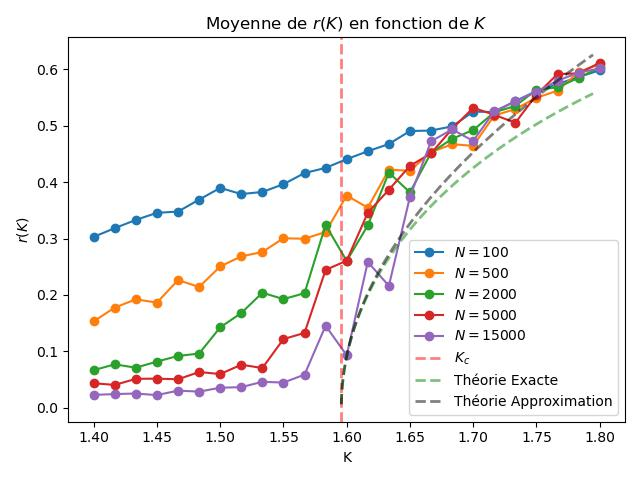
\includegraphics[width=\linewidth]{pics/kura9.jpg}
        \caption{}
        \label{fig:Kura9}
    \end{minipage} \hfill
    \begin{minipage}[c]{0.49\linewidth}
        \centering
        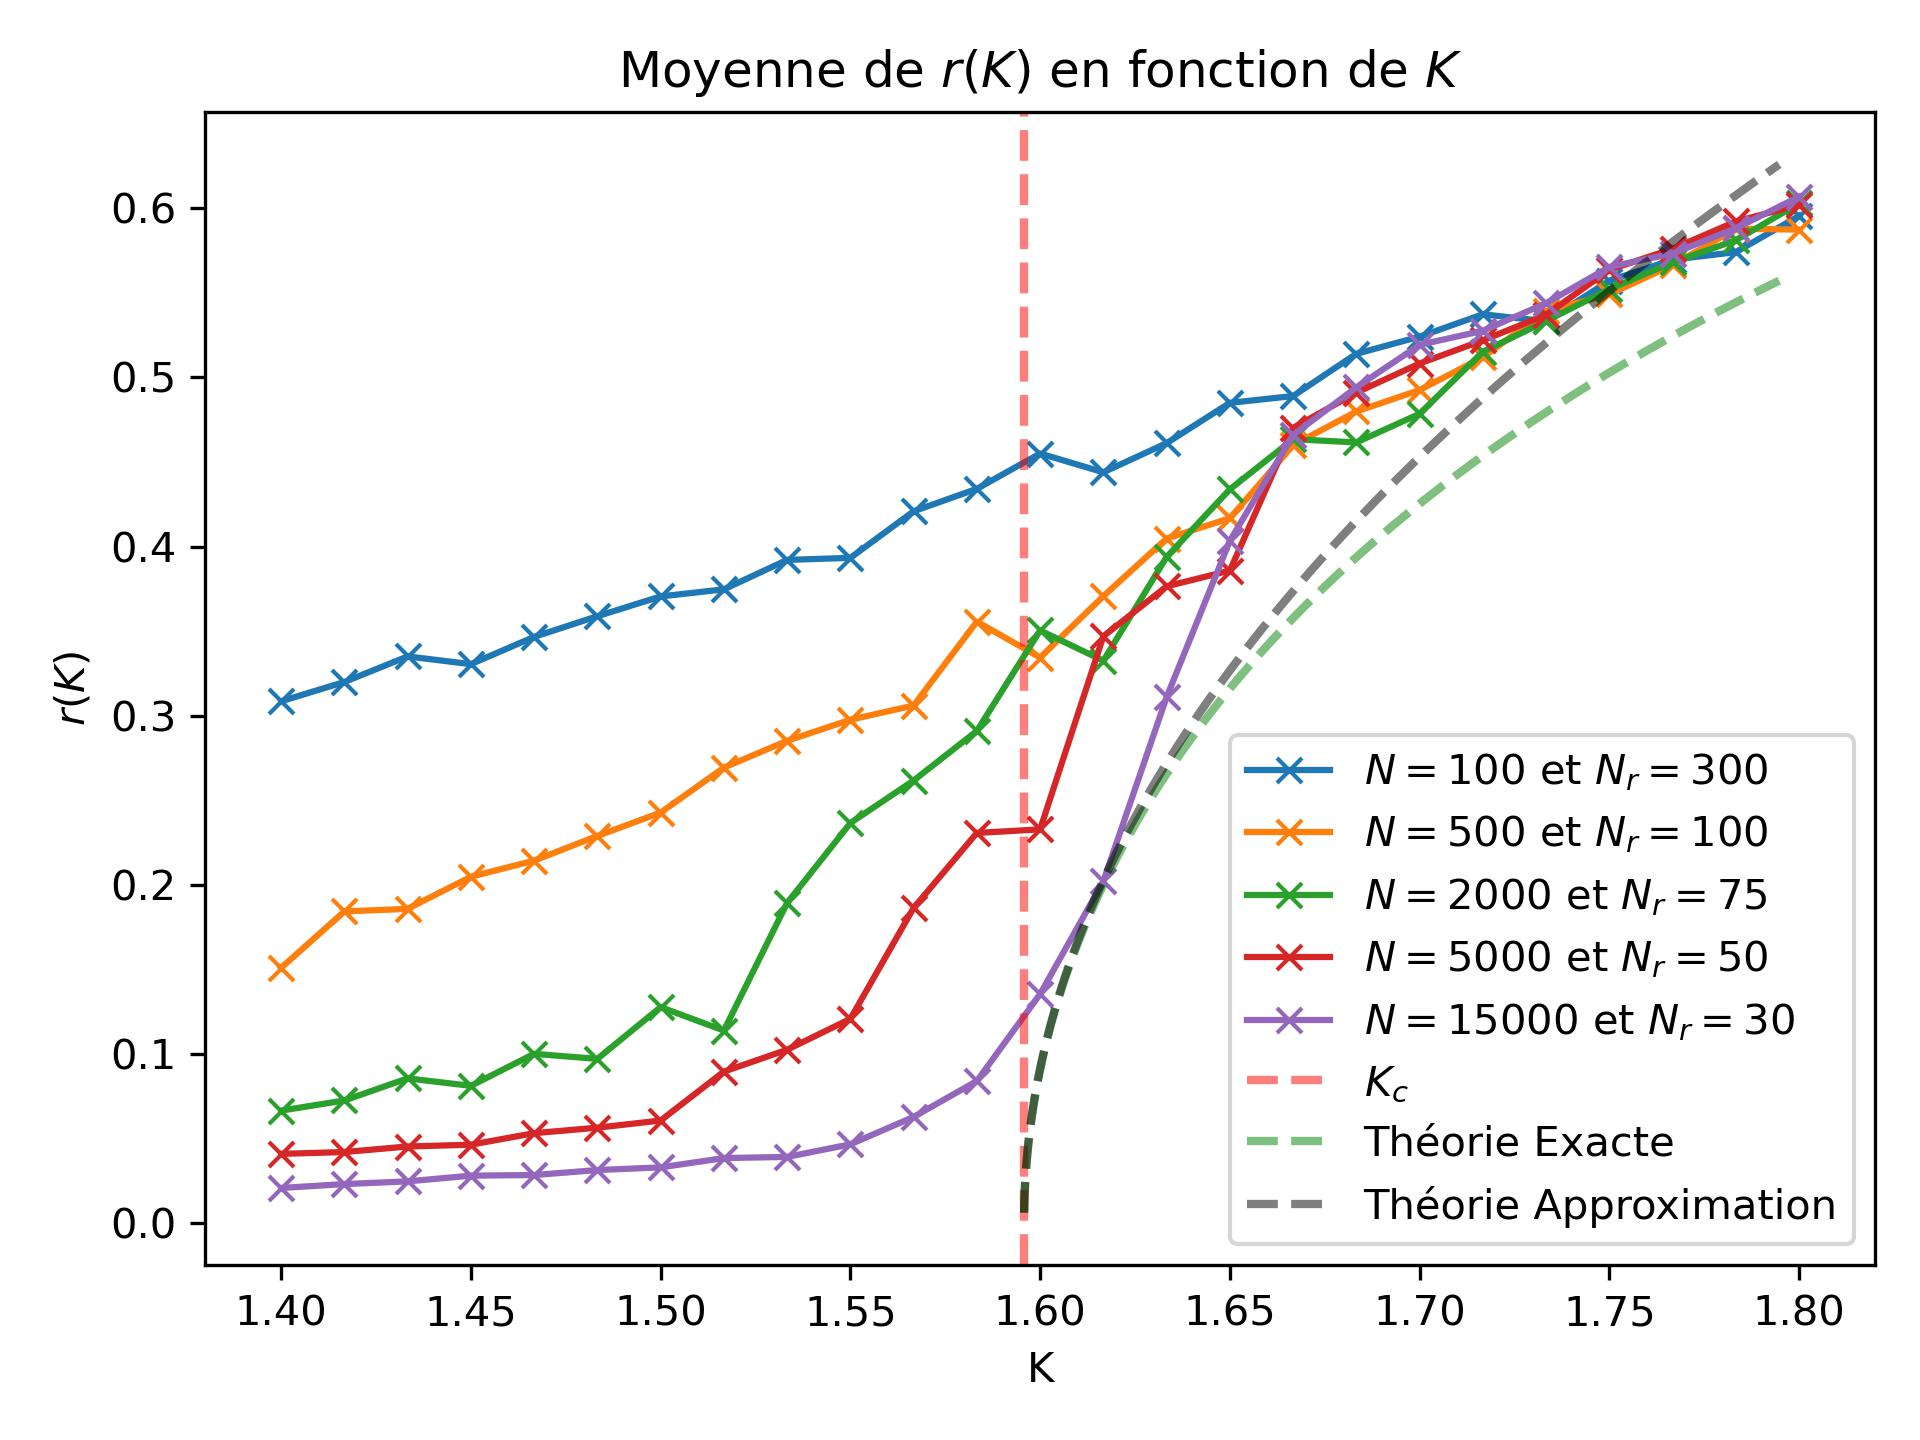
\includegraphics[width=\linewidth]{pics/kura9_good.jpg}
        \caption{}
        \label{fig:Kura9_good}
    \end{minipage}
\end{figure}

\section{Le modèle FPUT}
\subsection*{Question 1}
On a : 
\begin{align*}
    x_i &= a \sin(\frac{i \pi}N) \\ 
    V (x) &= \frac{x^2}2 + \alpha \frac{x^3}3
\end{align*}

Pour $N$ grand, on peut remplacer la somme des potentiels du Hamiltonien par la moyenne des valeurs des positions. On a donc deux termes : 
\begin{itemize}
    \item le terme à l'ordre deux : $<x^2> \propto <\sin^2> = \frac 12$
    \item le terme à l'ordre trois : $<x^3> \propto <\sin^3> = 0$
\end{itemize}

Le terme en alpha correspond au terme à l'ordre trois. Il est donc négligeable tant que $N$ est grand.

\begin{table}[H]
    \centering
    \begin{tabular}{|c | c | c |}
    \hline
         & $\alpha$ & Energie Total\\
    \hline\hline
        Système 1 & $0$ & $0.0770444$\\\hline
        Système 2 & $0.25$ & $0.0770444$\\
    \hline
    \end{tabular}
    \caption{Résultats FPUT 1}
    \label{tab:FPUT1}
\end{table}

\subsection*{Question 2}
Initialement, seul le mode de plus grande longueur d'onde (mode 1) est excité. Pour tout les autres modes, les énergies sont nulles. C'est un comportement induit par la non linéairité du système.
Or ce comportement a bien été prédit par la théorie de l'évolution des modes de Mary Tsingou:
\begin{figure}[H]
    \centering
    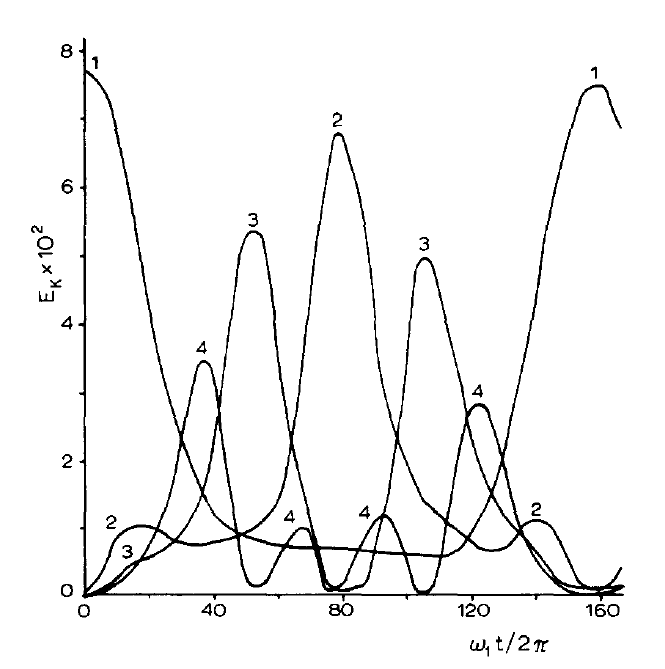
\includegraphics[scale=0.5]{pics/FPUT.png}
    \caption{Résultats de Mary Tsingou sur l’évolution des premiers modes normaux d’un
modèle FPUT}
    \label{fig:Mary_graph}
\end{figure}
\begin{table}[H]
    \centering
    \begin{tabular}{|c|c|c|}
    \hline
         & Système 1 & Système 2\\
         \hline \hline
        $\alpha$ & $0$ & $0.25$ \\\hline
        $E_0$ & $0.0$ & $0.0$ \\\hline
        $E_1$ & $0.0770444$ & $0.0770444$ \\\hline
        $E_2$ & $4.03151e-34$ & $4.03151e-34$ \\\hline
        $E_3$ & $4.43448e-34$ & $4.43448e-34$ \\
        \hline
    \end{tabular}
    \caption{Tableau des énergies des 4 premiers modes}
    \label{tab: energie_mode}
\end{table}

\subsection*{Question 3}
Pour $\alpha=0$, on ne distingue pas de fonctions de modes mais deux énergies $E=0$ et $E=7.6$ qui est l'énergie max du niveau excité. 
Pour $\alpha=0.25$, on obtient la figure de mode de Mary Tsingou avec l'état initial décrit dans la question 2, une évolution des modes qui tend à retourner dans l'état intial.
\begin{figure}[H]
    \centering
    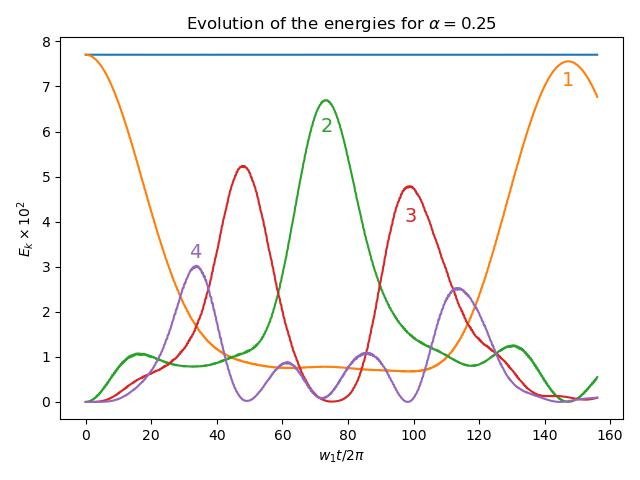
\includegraphics[width=0.75\linewidth]{pics/fput_0.25.jpg}
    \caption{Evolution temporelle de l'énergie des quatres premiers modes}
    \label{fig:Q3}
\end{figure}

\subsection*{Question 4}
On pourrait s'attendre à ce que l'énergie se disperse de manière plus uniforme dans les différents modes au fil du temps, plutôt que de revenir de manière significative vers le mode initial. C'est un comportement non intuitif et complexe, caractéristique des systèmes non linéaires.
\begin{figure}[H]
    \centering
    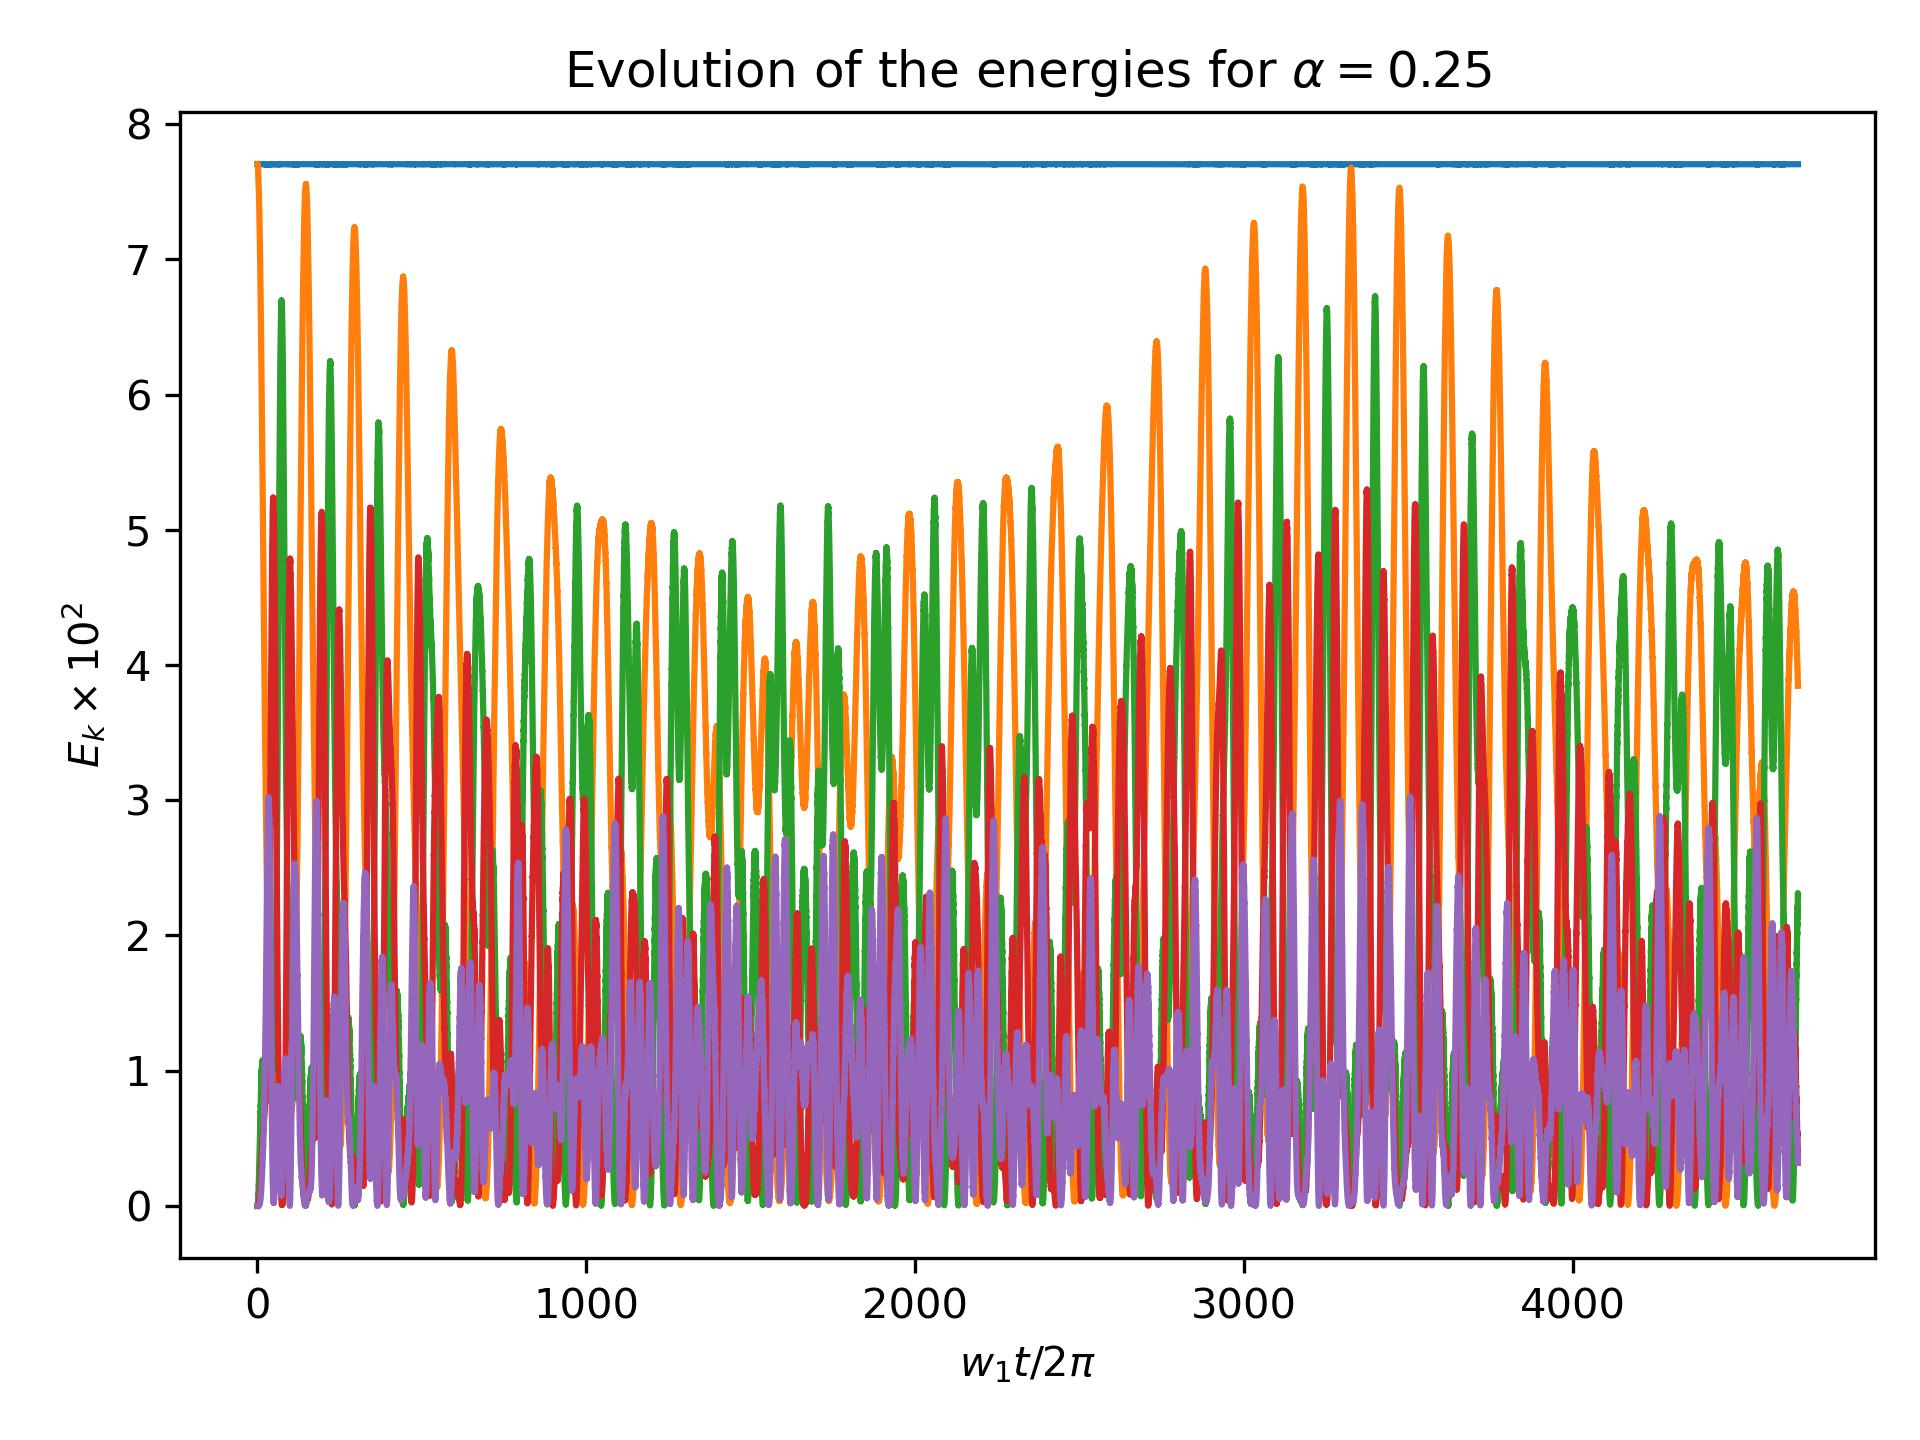
\includegraphics[width=0.75\linewidth]{pics/fput_long.jpg}
    \caption{Evolution temporelle de l'énergie des quatres premiers modes}
    \label{fig:Q4}
\end{figure}


\end{document}
